\documentclass[9pt]{beamer}

\usepackage{amsmath, amssymb}
\usepackage{fancyvrb, color, graphicx, hyperref, url}

\setbeamersize{text margin left=5pt, text margin right=5pt}

\setlength{\parskip}{\smallskipamount}
\setlength{\parindent}{0pt}

\usepackage{fontspec}
\setmonofont{DejaVu Sans Mono}

\usefonttheme[onlymath]{serif}

\usepackage{minted}
\newminted{python}{breaklines}
\newminted{julia}{breaklines}
\newminted{bash}{breaklines}
\newminted{text}{breaklines}

\newcommand{\txtinline}[1]{\mintinline{text}{#1}}
\newcommand{\pyinline}[1]{\mintinline{python}{#1}}
\newcommand{\jlinline}[1]{\mintinline{julia}{#1}}

\definecolor{mintedbg}{rgb}{0.90,0.90,0.90}
\usepackage{mdframed}

\BeforeBeginEnvironment{minted}{\begin{mdframed}[backgroundcolor=mintedbg,%
  rightline=false,leftline=false,topline=false,bottomline=false]}
\AfterEndEnvironment{minted}{\end{mdframed}}


\begin{document}

\title{Analisis Galat}
\subtitle{TF4062: Komputasi Rekayasa Lanjut}
\author{Iwan Prasetyo\\
Fadjar Fathurrahman}
\institute{
Teknik Fisika \\
Institut Teknologi Bandung
}
\date{}


\frame{\titlepage}


\begin{frame}
\frametitle{Galat dalam metode numerik}

Galat atau kesalahan (error) pada metode numerik muncul karena adanya aproksimasi
untuk merepresentasikan suatu kuantitas dan operasi matematik yang eksak.

Beberapa tipe galat:
\begin{itemize}
\item kesalahan pembulatan (rounding error): akibat penggunaan bilangan yang memiliki
  bilangan penting, jumlah digit, atau akurasi yang terbatas.
\item kesalahan pemotongan (truncation error): akibat adanya aproksimasi yang digunakan
  ketika merepresentasikan suatu prosedur matematika eksak.
\end{itemize}

Secara umum dapat dituliskan:
\begin{equation}
E_{t} = \text{true value} - \text{aproksimasi}
\end{equation}
di mana $E_t$ adalah nilai eksak dari galat ("true" error).

Galat lebih sering dinyatakan dalam nilai relatifnya:
\begin{equation}
\text{true fractional relative error} = \frac{\text{true error}}{\text{true value}}
\end{equation}
atau dalam persentase:
\begin{equation}
\epsilon_{t} = \frac{\text{true error}}{\text{true value}} 100\%
\end{equation}

\end{frame}


\begin{frame}
\frametitle{Sumber galat (error)}

Dalam banyak kasus kita tidak bisa mengetahui nilai sebenarnya (true value), sehingga
galat sebenarnya tidak dapat dihitung. Sebagai alternatif, digunakan galat aproksimasi:
\begin{equation}
\epsilon_{a} = \frac{\text{approximate error}}{\text{approximation}} 100\%
\end{equation}
Untuk metode iteratif sering digunakan:
\begin{equation}
\epsilon_{a} = \frac{\text{current approximation - prev approximation}}{\text{current approximation}} 100\%
\end{equation}

Salah satu tantangan yang sering muncul pada metode numerik adalah menentukan estimasi galat
tanpa adanya informasi mengenai informasi eksak.

\end{frame}


\begin{frame}
\frametitle{Kesalahan pembulatan (rounding error)}

Rounding error disebabkan karena komputer hanya menyimpan jumlah digit signifikan
yang tetap dan terbatas.
Bilangan-bilangan seperti $\pi$, $e$, dan $\sqrt{7}$ tidak bisa dinyatakan dengan jumlah
digit tetap.

Bilangan pada komputer dinyatakan dalam sistem biner.

Satuan dasar informasi pada komputer dinyatakan dalam \textit{word} yang terdiri dari
beberapa binary digit atau bit. Bilangan biasanya disimpan dalam beberapa word.

Ukuran dari 1 word biasanya bergantung dari jenis prosesor.

\end{frame}



\begin{frame}
\frametitle{Representasi bilangan integer}

Salah satu metode yang sering dipakai
adalah \textit{signed magnitude method}. Bit pertama digunakan untuk menyatakan
tanda (sign), 0 untuk bilangan positif dan 1 untuk bilangan negatif.
Bit yang lain digunakan untuk menyimpan bilangan.

\begin{figure}[H]
{\center
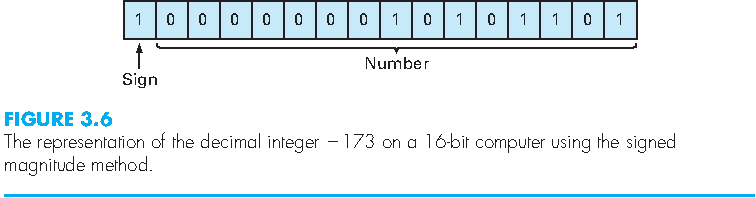
\includegraphics[scale=1.0]{images/Chapra_3_6.pdf}
\par}
\end{figure}

\end{frame}


\begin{frame}
\frametitle{Representasi floating-point}

Bilangan fraksional biasanya dinyatakan dalam bentuk floating point. Dengan pendekatan ini
suatu bilangan dinyatakan dalam bagian fraksional yang disebut mantissa atau significant
dan bagian integer yang disebut exponent atau characteristic:
\begin{equation}
m \cdot b^{e}
\end{equation}

$m$: mantissa

$b$: basis dari bilangan yang digunakan

$e$: exponent

\begin{figure}[H]
{\center
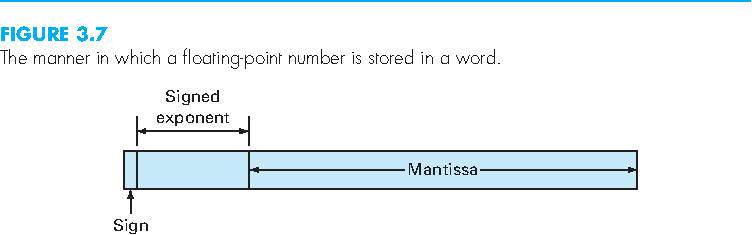
\includegraphics[scale=1.0]{images/Chapra_3_7.pdf}
\par}
\end{figure}

\end{frame}


\begin{frame}
\frametitle{Menghindari kesalahan pembulatan}

\begin{itemize}
\item menggunakan formula dengan kesalahan pembulatan yang lebih kecil.
\item menggunakan lebih banyak digit signifikan (extended precision).
\end{itemize}

\end{frame}


\begin{frame}
\frametitle{Kesalahan pemotongan (\textit{truncation error})}

Kesalahan pemotongan diakibatkan adanya aproksimasi dari suatu prosedur eksak.
Contohnya adalah pada pemotongan suku pada suatu deret tak hingga.

Contoh lain adalah kesalahan akibat adanya diskritisasi (\textit{discretization error})
dari proses yang kontinu seperti interpolasi, diferensiasi, dan integrasi.

Contoh lain adalah kesalahan konvergensi (\textit{convergence error}) dari suatu
metode iteratif. Banyak masalah nonlinear harus diselesaikan dengan metode iteratif.
Proses iteratif ini akan konvergen jika iterasi dilakukan terus sampai tak hingga.
Secara praktis hal ini tidak bisa dilakukan sehingga iterasi harus dihentikan dengan
jumlah terhingga.

\end{frame}



\begin{frame}
\frametitle{Sumber kesalahan yang lain}

\begin{itemize}
\item Kesalahan pada model matematika yang digunakan,
misalnya aproksimasi dari situasi fisis yang sebenarnya.
\item Kesalahan pada data input, misalnya dari pengukuran dengan akurasi yang terbatas.
\item Kesalahan manusia (pemrograman)
\end{itemize}


\end{frame}



\begin{frame}
\frametitle{Propagasi kesalahan}

Misalkan kita memiliki suatu fungsi $f(x)$ dengan variabel independen $x$ dan
$\tilde{x}$ adalah aproksimasi dari $x$. Kita ingin mengetahui perbedaan antara
hasil evaluasi dari $f(x)$ dengan $f(\tilde{x})$:
\begin{equation}
\Delta f(\tilde{x}) = \left| f(x) - f(\tilde{x}) \right|
\end{equation}
Gunakan deret Taylor:
\begin{equation}
f(x) = f(\tilde{x}) + f'(\tilde{x})(x - \tilde{x}) + \frac{f''(\tilde{x})}{2}(x - \tilde{x})^2 + \cdots
\end{equation}
Abaikan suku dengan turunan kedua ke atas:
\begin{equation}
f(x) - f(\tilde{x}) \approx f'(\tilde{x})(x - \tilde{x})
\end{equation}
atau:
\begin{equation}
\Delta f(\tilde{x}) = \left| f'(\tilde{x}) \right| \Delta \tilde{x}
\end{equation}

\end{frame}


\begin{frame}
\frametitle{Propagasi kesalahan}

Untuk fungsi multivariabel $f(x_{1},x_{2}, \ldots, x_{n})$:
\begin{equation}
\Delta f(\tilde{x}_{1}, \tilde{x}_{2}, \ldots, \tilde{x}_{n})
\approx
\left|\frac{\partial f}{\partial x_{1}} \right| \Delta\tilde{x}_{1} +
\left|\frac{\partial f}{\partial x_{2}} \right| \Delta\tilde{x}_{2} + \ldots
\left|\frac{\partial f}{\partial x_{n}} \right| \Delta\tilde{x}_{n}
\end{equation}

\begin{figure}[H]
{\center
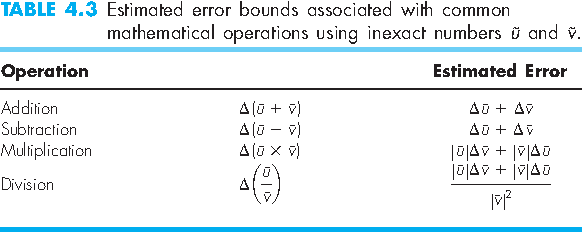
\includegraphics[width=\textwidth]{images/Chapra_table_4_3.pdf}
\par}
\end{figure}

\end{frame}


\begin{frame}
\frametitle{Stabilitas dan kondisi}

Kondisi dari suatu masalah matematika berhubungan dengan sensitivitas terhadap
perubahan pada nilai input.

Suatu algoritma atau komputasi dinyatakan tidak stabil secara numerik
(\textit{numerically unstable}) apabila ketidakpastian dari nilai input diperbesar
oleh metode numerik.

Dari deret Taylor orde 1:
\begin{equation}
f(x) = f(\tilde{x}) + f'(\tilde{x})(x - \tilde{x})
\end{equation}
Kesalahan relatif dari $f(x)$ didefinisikan sebagai:
\begin{equation}
\frac{f(x) - f(\tilde{x})}{f(\tilde{x})} = \frac{ f'(\tilde{x})(x - \tilde{x})}{f(\tilde{x})}
\end{equation}
Kesalahan relatif dari $x$:
\begin{equation}
\frac{x - \tilde{x}}{\tilde{x}}
\end{equation}
Bilangan kondisi untuk operasi $f(x)$ dapat didefinisikan sebagai rasio dari dua kesalahan tersebut:
\begin{equation}
\text{condition number} = \frac{\tilde{x} f'(\tilde{x})}{f(\tilde{x})}
\end{equation}


\end{frame}


\begin{frame}
\frametitle{Stabilitas dan kondisi}

\begin{equation}
\text{condition number} = \frac{\tilde{x} f'(\tilde{x})}{f(\tilde{x})}
\end{equation}

\begin{itemize}
\item Bilangan kondisi memberikan suatu ukuran seberapa besar ketidakpastian pada $x$
diperbesar oleh $f(x)$.
\item Nilai lebih kecil dari satu menyatakan bahwa kesalahan relatif mengalami atenuasi
(semakin kecil)
\item Nilai lebih besar dari satu menyatakan bawah kesalahan relatif mengalami amplifikasi
(semakin besar)
\end{itemize}

Suatu fungsi atau prosedur dengan nilai bilangan kondisi sangat besar sering disebut
\textit{ill-conditioned}.

\end{frame}


\end{document}
